%%%%%%%%%%%%%%%%%%%%%%%%%%%%%%%%%%%%%%%%%%%%%%%%%%%%%%%%%%%%%%%%%%%%%%%%%%%%%%%%%%%%%
% PACOTES                                                                           %
%%%%%%%%%%%%%%%%%%%%%%%%%%%%%%%%%%%%%%%%%%%%%%%%%%%%%%%%%%%%%%%%%%%%%%%%%%%%%%%%%%%%%
\documentclass[a4paper,11pt]{article}

%-----------------------------------------------------------------------------------%
% LAYOUT DA PÁGINA                                                                  %
%-----------------------------------------------------------------------------------%
\usepackage[top=2.25cm, bottom=2.25cm, left=2.25cm, right=2.25cm]{geometry}
%\usepackage{fancyhdr} % Permite controlar como são exibidos os cabeçalhos

%-----------------------------------------------------------------------------------%
% FORMATAÇÃO DO TEXTO                                                               %
%-----------------------------------------------------------------------------------%
%\usepackage{setspace} % Permite definir o espaçamento entre linhas

%-----------------------------------------------------------------------------------%
% PACOTES DE IMAGENS                                                                %
%-----------------------------------------------------------------------------------%
\usepackage[pdftex]{graphicx}
\pdfsuppresswarningpagegroup=1 % A warning issued when several PDF images are
% imported in the same page. Mostly harmless, can be almost always supressed.
%\usepackage[pstarrows]{pict2e} % Amplia as funcionalidades do ambiente picture
\usepackage{tikz}
\usetikzlibrary{shapes, arrows, arrows.meta}

%-----------------------------------------------------------------------------------%
% PACOTES DE TABELAS                                                                %
%-----------------------------------------------------------------------------------%
\usepackage{array} % Facilita a formatação de tabelas
%\usepackage{multirow} % Permite criar células que ocupam várias linhas em uma tabela
\usepackage{longtable} % Permite criar tabelas que quebram de página
\usepackage{booktabs}

%-----------------------------------------------------------------------------------%
% PACOTES MATEMÁTICOS DE BASE                                                       %
%-----------------------------------------------------------------------------------%
\usepackage{amsfonts,amstext,amscd,bezier,amsthm,amssymb}
\usepackage[centertags]{amsmath}

%-----------------------------------------------------------------------------------%
% PACOTES DE SÍMBOLOS MATEMÁTICOS                                                   %
%-----------------------------------------------------------------------------------%
\usepackage{mathtools} % Símbolos matemáticos extras. (ex.: \xrightharpoon)
%\usepackage[integrals]{wasysym} % Muda o estilo das integrais, além de outros
%                                 símbolos extras
%\usepackage[nice]{nicefrac} % Permite o uso de frações "melhores". Usar \nicefrac{}{}

%-----------------------------------------------------------------------------------%
% PACOTES DE FONTES MATEMÁTICAS                                                     %
%-----------------------------------------------------------------------------------%
%\usepackage{mathbbol} % Quase todos os símbolos com \mathbb
%\usepackage{bbm} % Extensão dos símbolos de \mathbb. Usar comando \mathbbm
%\usepackage{calrsfs} % Muda o estilo de \mathcal
%\usepackage[mathcal]{euscript} % Muda o estilo de \mathcal

%-----------------------------------------------------------------------------------%
% PACOTES DE CODIFICAÇÃO DE FONTES                                                  %
%-----------------------------------------------------------------------------------%
\usepackage[utf8]{inputenc} % Permite o uso de caracteres ISO 8859-1, incluindo os
%                               caracteres acentuados diretamente.
\usepackage[T1]{fontenc} % Uso de fontes T1, necessário para tratar caracteres
%                          acentuados como um único bloco.

%-----------------------------------------------------------------------------------%
% PACOTES DE LÍNGUAS                                                                %
%-----------------------------------------------------------------------------------%
\usepackage[french]{babel} % Seleciona a língua do documento, definindo nomes de
%                              seções, nome do índice, da bibliografia, etc. Em caso
%                              de documento com mais de uma língua, a padrão é a
%                              última.
\NoAutoSpaceBeforeFDP % Utilizar em francês se quiser evitar espaços antes de :

%-----------------------------------------------------------------------------------%
% PACOTES DE BIBLIOGRAFIA                                                           %
%-----------------------------------------------------------------------------------%
%\usepackage{babelbib} % Permite definir a língua das entradas da bibliografia. Usar
%                       [fixlanguage] para uma mesma língua para todas as entradas e
%                       \selectbiblanguage{} para definir a língua. Um estilo compa-
%                       tível com babelbib deve ser usado (ex: babplain)
\usepackage{cite} % Organiza os elementos citados dentro de um mesmo \cite.

%-----------------------------------------------------------------------------------%
% PACOTES DE FONTES                                                                 %
%-----------------------------------------------------------------------------------%
% Computer Modern (fonte padrão)                                                    %
% - - - - - - - - - - - - - - - - - - - - - - - - - - - - - - - - - - - - - - - - - %
%\usepackage{ae} % A usar com a fonte padrão do LaTeX quando forem gerados PDFs, para
%                 corrigir erros de visualização

% Computer Modern Bright (sans serif)                                               %
% - - - - - - - - - - - - - - - - - - - - - - - - - - - - - - - - - - - - - - - - - %
%\usepackage{cmbright}

% Times New Roman                                                                   %
% - - - - - - - - - - - - - - - - - - - - - - - - - - - - - - - - - - - - - - - - - %
%\usepackage{mathptmx} % Muda texto e modo matemático
%\usepackage{times} % Apenas texto, não muda modo matemático

% Arial                                                                             %
% - - - - - - - - - - - - - - - - - - - - - - - - - - - - - - - - - - - - - - - - - %
%\usepackage[scaled]{uarial} % Arial como fonte sans serif padrão

% Palatino                                                                          %
% - - - - - - - - - - - - - - - - - - - - - - - - - - - - - - - - - - - - - - - - - %
%\usepackage{mathpazo} % Muda texto e modo matemático
%\usepackage{palatino} % Apenas texto, não muda modo matemático

% Concrete                                                                          %
% - - - - - - - - - - - - - - - - - - - - - - - - - - - - - - - - - - - - - - - - - %
%\usepackage{ccfonts} % Texto: Concrete; Matemático: Concrete Math
%\usepackage{ccfonts, eulervm} % Texto: Concrete; Matemático: Euler

% Iwona                                                                             %
% - - - - - - - - - - - - - - - - - - - - - - - - - - - - - - - - - - - - - - - - - %
%\usepackage[math]{iwona} % Texto e modo matemático: Iwona

% Kurier                                                                            %
% - - - - - - - - - - - - - - - - - - - - - - - - - - - - - - - - - - - - - - - - - %
%\usepackage[math]{kurier} % Texto e modo matemático: Kurier

% Antykwa Póltawskiego                                                              %
% - - - - - - - - - - - - - - - - - - - - - - - - - - - - - - - - - - - - - - - - - %
%\usepackage{antpolt} % Texto: Antykwa Póltawskiego; Matemático: nenhum
                     % Usar fontenc = QX ou OT4

% Utopia                                                                            %
% - - - - - - - - - - - - - - - - - - - - - - - - - - - - - - - - - - - - - - - - - %                     
%\usepackage{fourier} % Texto: Utopia; Matemático: Fourier

% KP Serif                                                                          %
% - - - - - - - - - - - - - - - - - - - - - - - - - - - - - - - - - - - - - - - - - %
\usepackage{kpfonts}

%-----------------------------------------------------------------------------------%
% CORES                                                                             %
%-----------------------------------------------------------------------------------%
\usepackage{color}
\definecolor{darkgreen}{rgb}{0,0.5,0}
\definecolor{darkmagenta}{rgb}{0.5,0,0.5}
\definecolor{darkgray}{rgb}{0.5,0.5,0.5}
\definecolor{darkblue}{rgb}{0.2,0.2,0.4}
\definecolor{darkred}{rgb}{0.6,0.15,0.15}
\definecolor{gray}{rgb}{0.65,0.65,0.65}
\definecolor{lightgray}{rgb}{0.8,0.8,0.8}
\definecolor{lightblue}{rgb}{0.5,0.5,1}
\definecolor{lightgreen}{rgb}{0.5,1,0.5}
\definecolor{deadred}{rgb}{0.7, 0.2, 0.2}
\definecolor{deadblue}{rgb}{0.2, 0.2, 0.7}

%-----------------------------------------------------------------------------------%
% PACOTES DIVERSOS                                                                  %
%-----------------------------------------------------------------------------------%
\usepackage{icomma} % Permite uso de vírgula como separador decimal
\usepackage{url} % Pacote para não ter problemas com URLs. Usar \url{}
%\usepackage{randtext} % Troca a ordem de letras de uma frase (útil com e-mails em
                      % PDFs a serem publicados on-line.
\usepackage[hidelinks]{hyperref}
%\usepackage{showkeys} % Para mostrar o nome dos labels
\usepackage{enumitem} % Facilita o uso de listas, inclusive referências a itens de
                      % listas.
%\usepackage[absolute]{textpos} % Posição absoluta de texto na página
%\usepackage{pdfpages} % Permite incluir documentos em PDF no arquivo
%\usepackage{refcheck} % Verifica as referências procurando por
%                      % labels não usados ou equações numeradas sem labels.
%                      % Verificar o arquivo .log e procurar por RefCheck.
\usepackage[french, onelanguage]{algorithm2e}

%%%%%%%%%%%%%%%%%%%%%%%%%%%%%%%%%%%%%%%%%%%%%%%%%%%%%%%%%%%%%%%%%%%%%%%%%%%%%%%%%%%%%
% CONFIGURAÇÕES                                                                     %
%%%%%%%%%%%%%%%%%%%%%%%%%%%%%%%%%%%%%%%%%%%%%%%%%%%%%%%%%%%%%%%%%%%%%%%%%%%%%%%%%%%%%

%-----------------------------------------------------------------------------------%
% FORMATAÇÃO DO TEXTO                                                               %
%-----------------------------------------------------------------------------------%
%\onehalfspacing % Espaçamento 1 1/2 (definido no pacote setspace)

%-----------------------------------------------------------------------------------%
% DEFINIÇÃO DE AMBIENTES MATEMÁTICOS                                                %
%-----------------------------------------------------------------------------------%
\theoremstyle{plain}
\newtheorem*{prop}{Proposition}
\theoremstyle{definition}
\newtheorem*{defi}{Définition}
\newtheorem*{remk}{Remarque}

%-----------------------------------------------------------------------------------%
% DEFINIÇÃO DE COMANDOS MATEMÁTICOS                                                 %
%-----------------------------------------------------------------------------------%
%\newcommand*\diff{\mathop{}\!\mathrm{d}}

%\newcommand{\norm}[1]{\left\lVert #1\right\lVert} % Norma
%\newcommand{\abs}[1]{\left\lvert #1\right \rvert} % Valor absoluto
%\newcommand{\floor}[1]{\left\lfloor #1 \right\rfloor} % Arredondar para baixo
%\newcommand{\ceil}[1]{\left\lceil #1 \right\rceil} % Arredondar para cima
\DeclarePairedDelimiter{\ceil}{\lceil}{\rceil}
\DeclarePairedDelimiter{\floor}{\lfloor}{\rfloor}
\DeclarePairedDelimiter{\abs}{\lvert}{\rvert}
\DeclareMathOperator*{\argmax}{argmax}
\DeclareMathOperator*{\argmin}{argmin}
\DeclareMathOperator{\ECO}{ECO}
\DeclareMathOperator{\ECR}{ECR}
\DeclareMathOperator{\EC}{EC}
\DeclareMathOperator{\EVOI}{EVOI}

%-----------------------------------------------------------------------------------%
% NUMERAÇÃO DE ELEMENTOS                                                            %
%-----------------------------------------------------------------------------------%
%\numberwithin{table}{section}
%\numberwithin{table}{subsection}
%\numberwithin{figure}{section}
%\numberwithin{figure}{subsection}
%\numberwithin{equation}{section}
%\numberwithin{equation}{subsection}
%\numberwithin{theo}{chapter}
%\numberwithin{theo}{subsection}

% Maximal percentage of the page occupied by floats
\renewcommand\floatpagefraction{.9}
\renewcommand\topfraction{.9}
\renewcommand\bottomfraction{.9}
\renewcommand\textfraction{.1}
% Maximal number of floats per page
\setcounter{totalnumber}{50}
\setcounter{topnumber}{50}
\setcounter{bottomnumber}{50}

%%%%%%%%%%%%%%%%%%%%%%%%%%%%%%%%%%%%%%%%%%%%%%%%%%%%%%%%%%%%%%%%%%%%%%%%%%%%%%%%%%%%%
% ESTRUTURA DO DOCUMENTO                                                            %
%%%%%%%%%%%%%%%%%%%%%%%%%%%%%%%%%%%%%%%%%%%%%%%%%%%%%%%%%%%%%%%%%%%%%%%%%%%%%%%%%%%%%
\begin{document}

\setlist[itemize]{label=\textbullet, nosep}

\pagestyle{plain}

\title{Troubleshooting \\ Manuel d'utilisateur}
\author{Ariana Carnielli et Ivan Kachaikin}
\date{Encadrants~: Paolo Viappiani et Pierre-Henri Wuillemin}
\maketitle

Le logiciel est lancé avec la commande \texttt{python MainWindow.py}. La description du problème de \emph{Troubleshooting} à être résolu est chargée automatiquement à partir du fichier \texttt{ProblemDefinition.py}.

\begin{center}
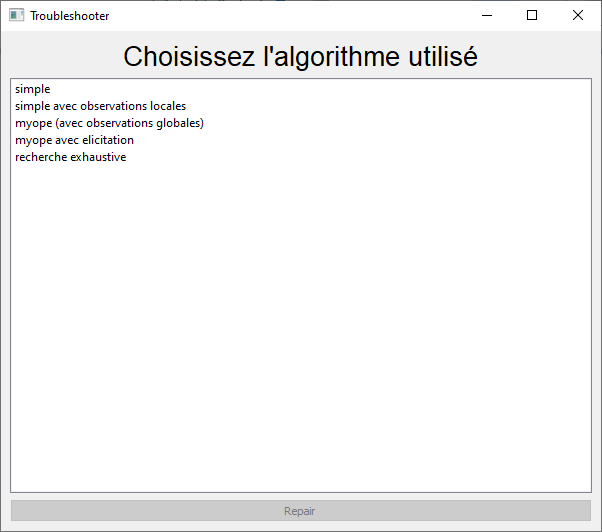
\includegraphics[scale=0.667]{Figures/tela_inicial.png}
\end{center}
L'écran d'accueil du logiciel permet de choisir l'algorithme à être utilisé pour la résolution du problème de Troubleshooting. Cinq algorithmes sont proposés~: l'algorithme simple, l'algorithme simple avec observations locales, l'algorithme myope (avec observations globales), l'algorithme myope avec élicitation et la recherche exhaustive.

\begin{center}
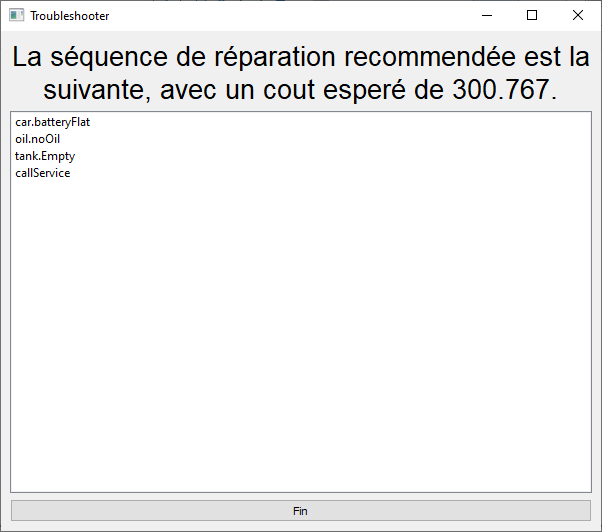
\includegraphics[scale=0.667]{Figures/algo_simples}
\end{center}
L'écran ci-dessus s'affiche suite au choix de l'algorithme simple. Il donne la séquence de réparations à réaliser et son coût espéré. Le bouton «~Fin~» permet de quitter le logiciel.

\begin{center}
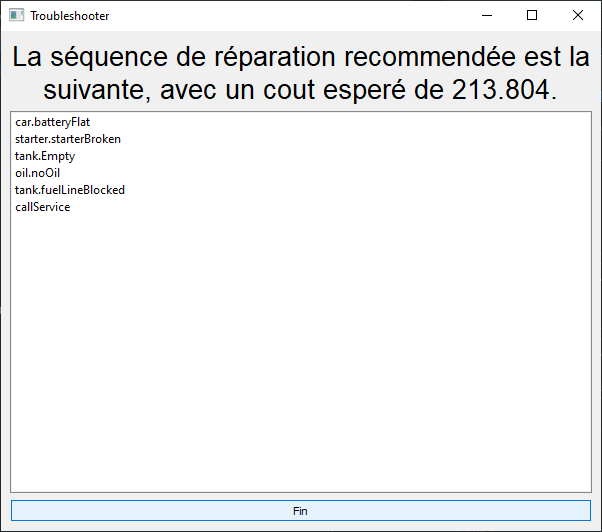
\includegraphics[scale=0.667]{Figures/algo_simples_obs}
\end{center}
Le comportement est similaire pour l'algorithme simple avec observations locales.

\begin{center}
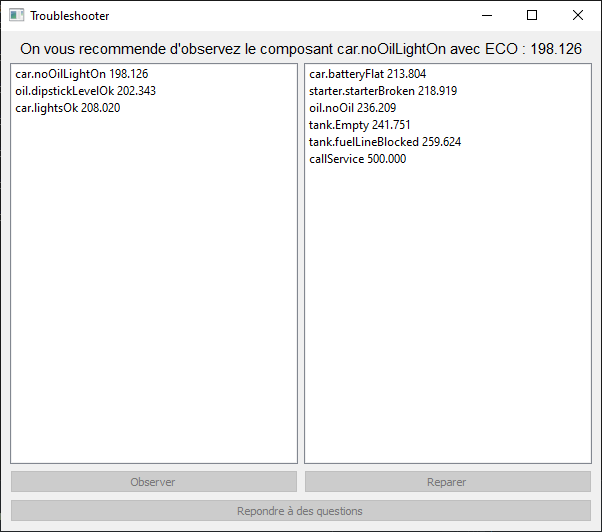
\includegraphics[scale=0.667]{Figures/myope_1}
\end{center}
La sélection de l'algorithme myope avec ou sans élicitation utilise un mode interactif, comme affiché sur l'écran ci-dessous. Il donne en haut l'action suggérée avec son coût espéré myope, mais permet une sélection de n'importe quelle action, affichant pour chacune d'entre elles son coût espéré myope. Les observations sont affichées sur la colonne de gauche et les réparations ou paires observation-réparation, sur la colonne de droite.

\begin{center}
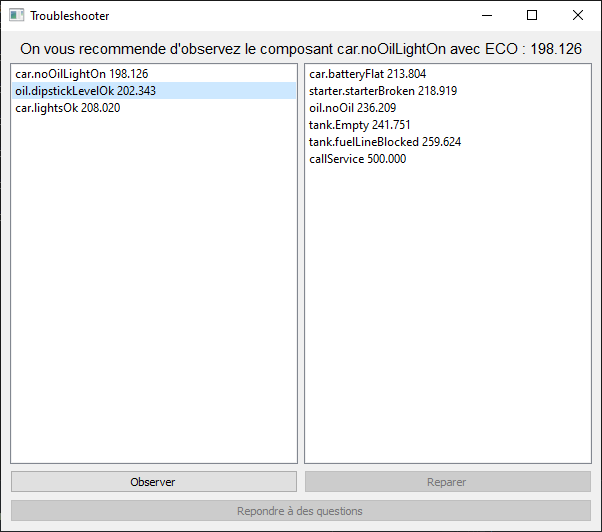
\includegraphics[scale=0.667]{Figures/myope_2}
\end{center}
La sélection d'une observation, comme sur la figure, active le bouton «~Observer~».

\begin{center}
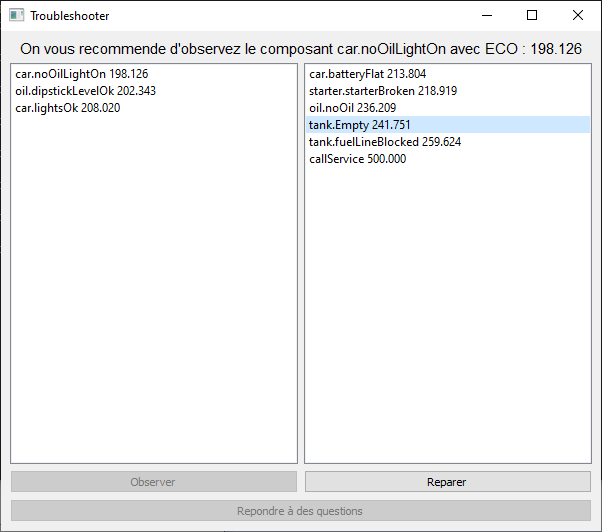
\includegraphics[scale=0.667]{Figures/myope_3}
\end{center}
Similairement, la sélection d'une réparation ou observation-réparation active le bouton «~Reparer~».

\begin{center}
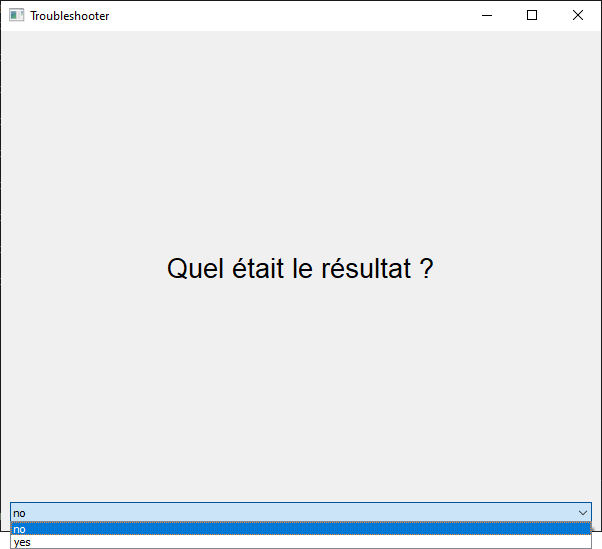
\includegraphics[scale=0.667]{Figures/observacao}
\end{center}
Lors de la sélection d'une observation et après un clic sur le bouton «~Observer~», on tombe sur l'écran ci-dessus, qui permet d'indiquer au logiciel quelle a été le résultat de l'observation. Après la sélection, le logiciel revient à l'écran de sélection d'action. Les actions qui ne sont plus disponibles ne sont plus affichées.

\begin{center}
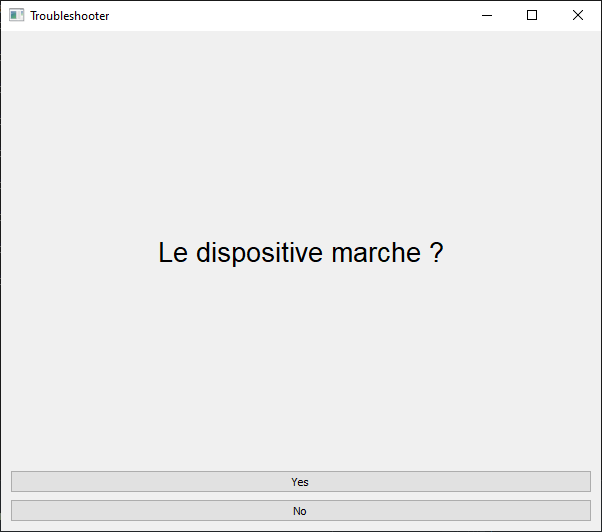
\includegraphics[scale=0.667]{Figures/reparacao}
\end{center}
Lors de la sélection d'une réparation et après un clic sur le bouton «~Reparer~», on tombe sur l'écran ci-dessus, qui permet d'indiquer au logiciel si la réparation a résolu le problème ou pas. En cas affirmatif, le logiciel se termine~; dans le cas contraire, on revient à l'écran de sélection d'actions.

\begin{center}
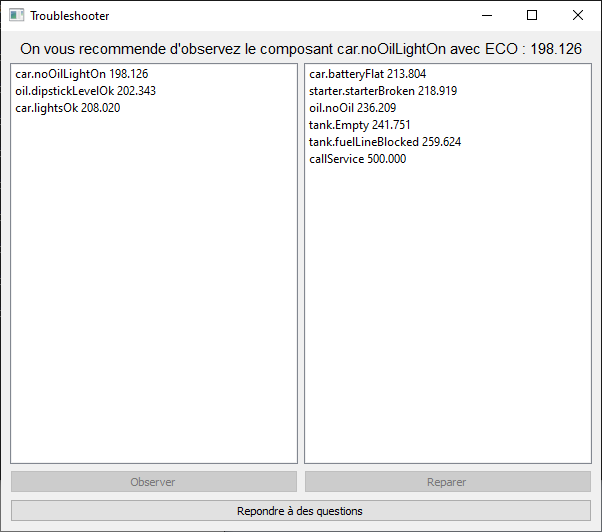
\includegraphics[scale=0.667]{Figures/elicitacao1}
\end{center}
Lorsque l'on choisit l'algorithme myope avec élicitation, le bouton «~Répondre à des questions~» en bas de l'écran est activé.

\begin{center}
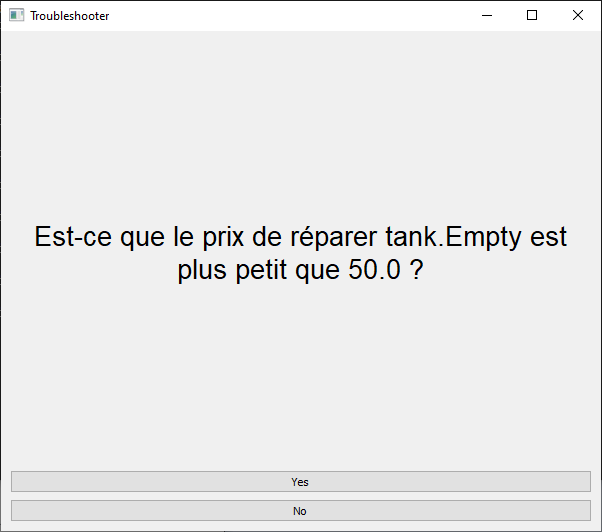
\includegraphics[scale=0.667]{Figures/elicitacao2}
\end{center}
Lorsqu'il y a des questions disponibles et que l'on clique sur ce bouton, il pose la meilleure question et permet à l'utilisateur de répondre. Suite à la réponse, le logiciel revient sur l'écran de sélection d'action. 

\begin{center}
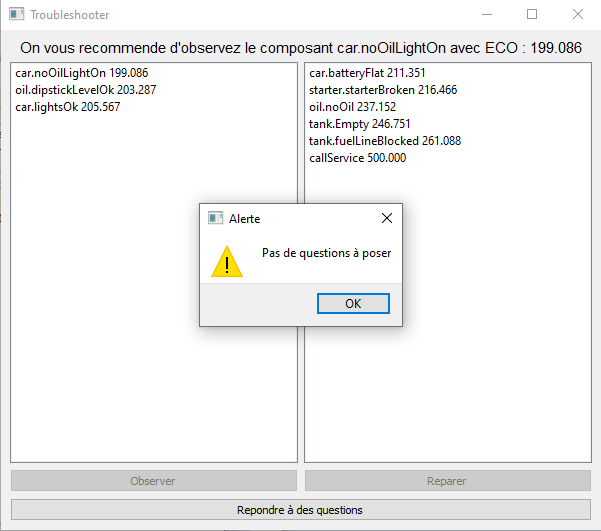
\includegraphics[scale=0.667]{Figures/elicitacao_sem_questoes}
\end{center}
Il se peut qu'il n'y ait pas de question intéressante à poser. Dans ce cas, un clic sur le bouton «~Répondre à des questions~» informe l'utilisateur par une fenêtre d'alerte.

\begin{center}
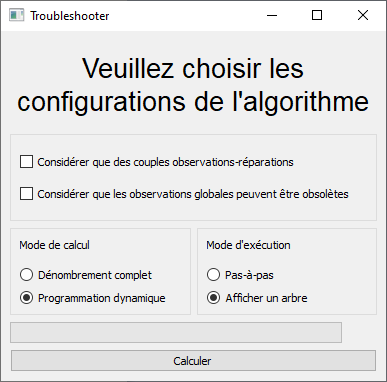
\includegraphics[scale=0.667]{Figures/exato_1}
\end{center}
Lorsque l'utilisateur choisit la résolution par recherche exhaustive, le premier écran permet de choisir des paramètres. Il est possible de ne considérer que des couples observation-réparation afin de simplifier les actions, ainsi que de choisir de prendre en compte le fait que les observations globales peuvent devenir obsolètes suite à des réparations. Le choix de l'algorithme utilisé (dénombrement complet, plus lent, et par programmation dynamique, plus rapide), est également proposé. Le choix du mode d'exécution permet de déterminer si, une fois la stratégie optimale calculée, elle sera affichée de façon interactive comme pour les autres algorithmes ou sous forme d'arbre, auquel cas le lecteur PDF par défaut de l'utilisateur est ouvert avec le fichier crée contenant l'arbre.

\begin{center}
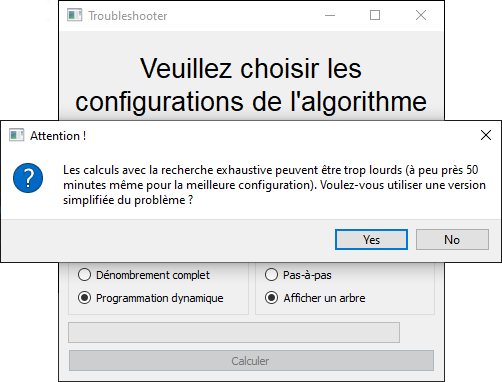
\includegraphics[scale=0.667]{Figures/exato_popup}
\end{center}
L'algorithme exact peut prendre longtemps à tourner. Un message alerte l'utilisateur de ce fait et lui propose d'utiliser plutôt une version simplifiée du problème de \emph{Troubleshooting} avec moins d'actions disponibles afin d'accélérer le calcul.

\begin{center}
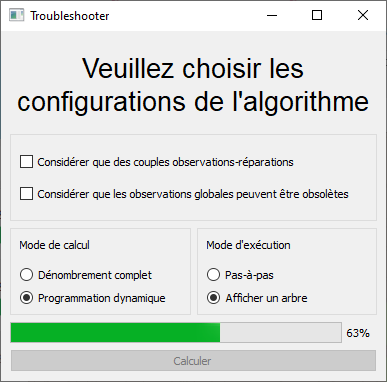
\includegraphics[scale=0.667]{Figures/exato_2}
\end{center}
L'algorithme exact peut prendre du temps, une barre permet de suivre la progression du calcul.

\begin{center}
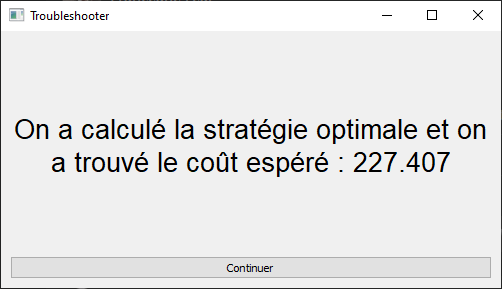
\includegraphics[scale=0.667]{Figures/exato_3_arvore1}
\end{center}
À la fin du calcul de la stratégie optimale, quel que soit le mode d'exécution choisi, le coût espéré de réparation est affiché.

\clearpage

\begin{center}
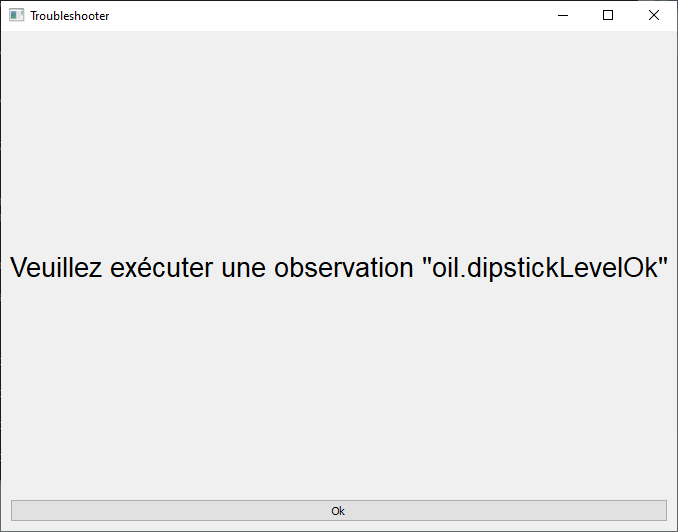
\includegraphics[scale=0.667]{Figures/exato_3_pas_a_pas1}
\end{center}
Dans le mode «~Pas-à-pas~», contrairement au mode interactif des algorithmes myopes, il n'est pas possible de choisir une action différente de celle proposée par l'algorithme. L'action proposée est affichée et des écrans demandant son résultat, similaires à ceux du cas myope, sont présentés.

\begin{center}
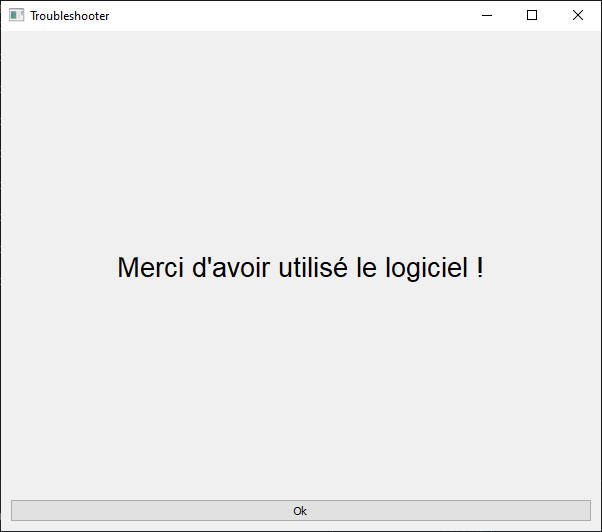
\includegraphics[scale=0.667]{Figures/fim}
\end{center}

\end{document}
